\documentclass[10pt]{beamer}
\usepackage[utf8]{inputenc}
\usepackage{graphicx}
\usepackage{listings}
\usepackage{minted}
\usepackage{multicol}
\usepackage {mathtools}
\usetheme{CambridgeUS}
\usecolortheme{dolphin}

% set colors
\definecolor{myNewColorA}{RGB}{0, 55, 158}
\definecolor{myNewColorB}{RGB}{0, 55, 158}
\definecolor{myNewColorC}{RGB}{0, 55, 158}
\setbeamercolor*{palette primary}{bg=myNewColorC, fg = white}
\setbeamercolor*{palette secondary}{bg=myNewColorB, fg = white}
\setbeamercolor*{palette tertiary}{bg=myNewColorA, fg = white}
\setbeamercolor*{titlelike}{fg=myNewColorA}
\setbeamercolor*{title}{bg=myNewColorA, fg = white}
\setbeamercolor*{item}{fg=myNewColorA}
\setbeamercolor*{caption name}{fg=myNewColorA}
\usefonttheme{professionalfonts}
\usepackage{natbib}
\usepackage{hyperref}

\newcommand{\specialcell}[2][c]{%
  \begin{tabular}[#1]{@{}c@{}}#2\end{tabular}}
  
\lstdefinelanguage{Kotlin}{
  comment=[l]{//},
  commentstyle={\color{gray}\ttfamily},
  emph={filter, first, firstOrNull, forEach, lazy, map, mapNotNull, println},
  emphstyle={\color{OrangeRed}},
  identifierstyle=\color{black},
  keywords={!in, !is, abstract, actual, annotation, as, as?, break, by, catch, class, companion, const, constructor, continue, crossinline, data, delegate, do, dynamic, else, enum, expect, external, false, field, file, final, finally, for, fun, get, if, import, in, infix, init, inline, inner, interface, internal, is, lateinit, noinline, null, object, open, operator, out, override, package, param, private, property, protected, public, receiveris, reified, return, return@, sealed, set, setparam, super, suspend, tailrec, this, throw, true, try, typealias, typeof, val, var, vararg, when, where, while},
  keywordstyle={\color{NavyBlue}\bfseries},
  morecomment=[s]{/*}{*/},
  morestring=[b]",
  morestring=[s]{"""*}{*"""},
  ndkeywords={@Deprecated, @JvmField, @JvmName, @JvmOverloads, @JvmStatic, @JvmSynthetic, Array, Byte, Double, Float, Int, Integer, Iterable, Long, Runnable, Short, String, Any, Unit, Nothing},
  ndkeywordstyle={\color{BurntOrange}\bfseries},
  sensitive=true,
  stringstyle={\color{ForestGreen}\ttfamily},
}

\setminted[kotlin]{
  linenos=true,
  breaklines=true,
  autogobble,
  encoding=utf8,
  fontsize=\footnotesize,
  frame=lines
}

%------------------------------------------------------------
%\titlegraphic{\includegraphics[height=1.5cm]{download.png}} 

\setbeamerfont{title}{size=\large}
\setbeamerfont{subtitle}{size=\small}
\setbeamerfont{author}{size=\small}
\setbeamerfont{date}{size=\small}
\setbeamerfont{institute}{size=\small}
\title[MaggioliEbook]{Utilizzo delle pratiche DevOps nel processo di sviluppo delle applicazioni mobile - MaggioliEbook}

\institute[0000926989]{Alma Mater Studiorum - Università di Bologna \\ Campus di Cesena \\ Laboratorio di Sistemi Software}
\author[Filippo Paganelli]{Filippo Paganelli \\ 0000926989 \\ filippo.paganelli3@studio.unibo.it}
\date[\textcolor{white}{A.A. 21/22} ]
{A.A. 21/22}

%------------------------------------------------------------
%This block of commands puts the table of contents at the 
%beginning of each section and highlights the current section:
\AtBeginSection[]
{
  \begin{frame}
    \frametitle{Contents}
    \tableofcontents[currentsection]
  \end{frame}
}

%\AtBeginSection[]{
%  \begin{frame}
%  \vfill
%  \centering
%  \begin{beamercolorbox}[sep=8pt,center,shadow=true,rounded=true]{title}
%    \usebeamerfont{title}\insertsectionhead\par%
%  \end{beamercolorbox}
%  \vfill
%  \end{frame}
%}
%------------------------------------------------------------

\begin{document}

%The next statement creates the title page.
\frame{\titlepage}
\begin{frame}
\frametitle{Contents}
\tableofcontents
\end{frame}
%------------------------------------------------------------
% !TeX root = ../main.tex

\section{Overview}
    \begin{frame}{Overview}
        \begin{itemize}
            \item Goal CI/CD
                \begin{itemize}
                    \item Progettazione di un processo automatizzato per lo sviluppo di applicazioni mobile adottando tecniche e pratiche della metodologia DevOps.
                    \item Progettazione del processo in modo tale da poter essere utilizzato dai reparti aziendali che si occupano di applicazioni mobile.
                \end{itemize}
            \item Goal Applicazione MaggioliEbook
                \begin{itemize}
                    \item Sviluppo di un lettore per i documenti digitali pubblicati da Maggioli Editore.
                    \item Dimostrazione dell'efficacia del processo progettato.
                    \item Utilizzo del framework cross-platform Kotlin Multiplatform Mobile.
                \end{itemize}
        \end{itemize}
    \end{frame}

% !TeX root = ../main.tex

\section{CI/CD}
    \begin{frame}{Mobile Application Development Lifecycle}
        Per poter automatizzare un processo è necessario prima comprendere da quali task è composto e le relazioni tra di essi:
        \begin{columns}[onlytextwidth]
            \begin{column}{0.4\textwidth}
                \begin{itemize}
                    \item Pianificazione
                    \item Progettazione
                    \item Sviluppo
                    \item Stabilizzazione
                    \item Release
                    \item Monitoring
                \end{itemize}
            \end{column}
            \begin{column}{0.6\textwidth}
                \begin{figure}[H]
                    \centering
                    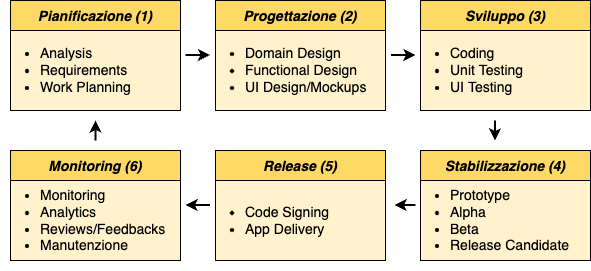
\includegraphics[width=1\textwidth]{img/tesi-2-Page-9.drawio.png}
                \end{figure}    
            \end{column}
       \end{columns}
    \end{frame}


%    \begin{frame}{Pipeline Obiettivo}
%        \begin{itemize}
%            \item I task del processo a cui sono applicate le tecniche di Continuous Integration e Continuous Delivery sono \textit{Sviluppo}, \textit{Stabilizzazione} e \textit{Release}.
%            \item Non esiste il concetto di deployment automatizzato nel mondo delle applicazioni mobile: l'applicazione viene rilasciata tramite pubblicazione sull'apposito store e l'utente effettua in un secondo momento l'installazione sul proprio dispositivo.
%            \item Dato il vincolo tecnologico del framework KMM per lo sviluppo della applicazione, la pipeline è stata progettata utilizzando come caso d'uso l'applicazione base generata con il plugin Gradle KMM.
%        \end{itemize}
%    \end{frame}

    \begin{frame}{Branching Model}
        \begin{columns}[onlytextwidth]
            \begin{column}{0.5\textwidth}
                \begin{itemize}
                    \item Fondamentale per l'efficacia del processo progettato
                    \item Basato su GitFlow
                    \item 3 branch principali:
                    \begin{itemize}
                        \item \textit{dev} (alpha)
                        \item \textit{test} (beta)
                        \item \textit{main} (prod)
                    \end{itemize}
                \end{itemize}
            \end{column}
            \begin{column}{0.5\textwidth}
                \begin{figure}[H]
                    \centering
                    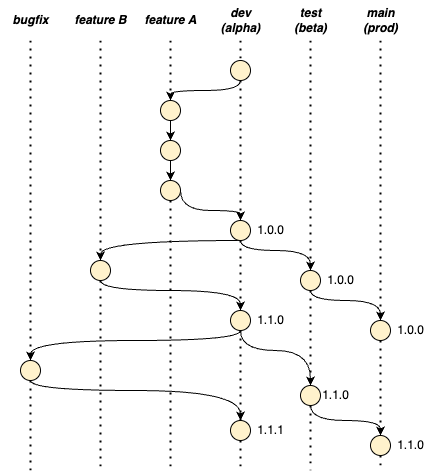
\includegraphics[width=1\textwidth]{img/tesi-13-branching.drawio.png}
                \end{figure}
            \end{column}
        \end{columns}
    \end{frame}
    
    \begin{frame}{Pipeline Obiettivo}
        \begin{figure}[H]
            \centering
            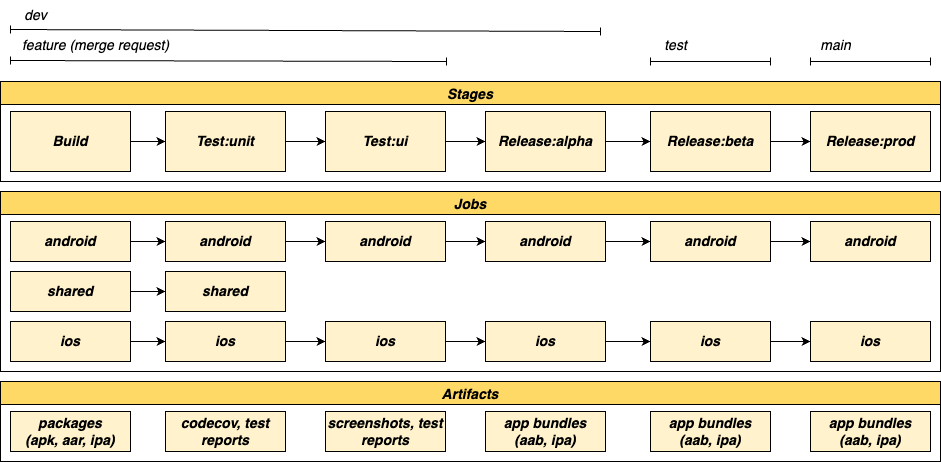
\includegraphics[width=1\textwidth]{img/tesi-2-Page-12.drawio.png}
        \end{figure}  
    \end{frame}

    \begin{frame}{Continuous Integration}
        \begin{itemize}
            \item \textbf{Build} - Fase di compilazione e packaging.
            \item \textbf{Test}
            \begin{itemize}
                \item \textit{Unit Testing} - Fase di testing della business logic.
                \item \textit{UI Testing} - Fase di testing della interfaccia grafica.
            \end{itemize}
        \end{itemize}
    \end{frame}

    \begin{frame}{Continuous Delivery}
        \begin{itemize}
            \item \textbf{Release}
            \begin{itemize}
                \item \textit{Alpha} - Fase di rilascio a scopo di test interno.
                \item \textit{Beta} - Fase di rilascio a scopo di test esterno.
                \item \textit{Prod} - Fase di rilascio a scopo di pubblicazione sugli store.
            \end{itemize}
        \end{itemize}
    \end{frame}

    \begin{frame}{Continuous Inspection}
        \begin{columns}[onlytextwidth]
            \begin{column}{0.4\textwidth}
                \begin{itemize}
                    \item \textbf{Test}
                        \begin{itemize}
                            \item \textit{Unit Testing} - Fase di testing della business logic.
                            \item \textit{UI Testing} - Fase di testing della interfaccia grafica.
                        \end{itemize}
                    \item \textbf{Analysis}
                        \begin{itemize}
                            \item \textit{SAST} - Fase di analisi statica del codice.
                            \item \textit{SCA} - Fase di analisi delle dipendenze.
                            \item \textit{Sonar} - Fase di upload dei report su SonarQube.
                        \end{itemize}
                \end{itemize}
            \end{column}
            \begin{column}{0.6\textwidth}
                \begin{figure}[H]
                    \centering
                    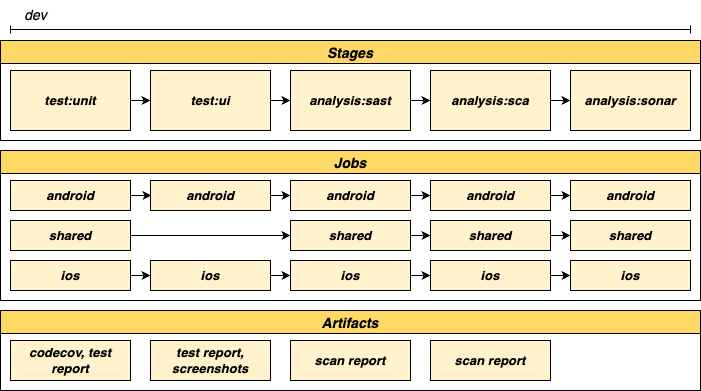
\includegraphics[width=1\textwidth]{img/tesi-2-Page-19.drawio.png}
                \end{figure}
            \end{column}
            
        \end{columns}
    \end{frame}

% !TeX root = ../main.tex

\section{MaggioliEbook}
    \begin{frame}{Introduzione}
        \begin{itemize}
            \item Applicazione Mobile realizzata come caso d'uso della CI/CD progettata.
            \item PoC interno del reparto Ricerca e Sviluppo.
            \item Sono coinvolte figure interne esperte di dominio nelle fasi:
            \begin{itemize}
                \item Analisi dei requisiti
                \item Progettazione (modellazione del dominio)
                \item Testing esterno (versione beta)
            \end{itemize}
            \item Dominio: Editoria Digitale
        \end{itemize}
    \end{frame}

    \begin{frame}{Requisiti}
        \begin{itemize}
            \item \textbf{Requisiti Funzionali}
            \begin{itemize}
                \item Visualizzazione documenti statici e fluidi.
                \item Modifica documenti statici e fluidi.
                \begin{itemize}
                    \item Creazione, lettura ed eliminazione di segnalibri, annotazioni, evidenziazioni e sottolineature.
                \end{itemize}
                \item Ricerca documenti.
                \item Gestione preferiti.
                \item Autenticazione utenti abbonati.
            \end{itemize}
            \item \textbf{Requisiti Non Funzionali}
            \begin{itemize}
                \item Sviluppo nativo Android e iOS (Kotlin e Swift).
                \item Framework Kotlin Multiplatform Mobile.
                \item CI/CD con rilascio automatico.
            \end{itemize}
        \end{itemize}
    \end{frame}
    
    \begin{frame}{Ubiquitous Language}
        \begin{itemize}
            \item Glossario delle entità:
            \begin{itemize}
            \item \textit{Reader} - Lettore di documenti in grado di visualizzarlo ed interagire con esso.
            \item \textit{Documento} - Contenuto digitale pubblicato da Maggioli Editore.
            \item \textit{Documento Statico} - Documento con una certa struttura definita nel formato (PDF).
            \item \textit{Documento Fluido} - Documento senza struttura in grado di adattarsi al dispositivo in cui viene aperto (EPUB).
            \item \textit{Libro} - Tipologia principale di documento fluido.
            \item \textit{Rivista} - Tipologia principale di documento statico.
            \item \textit{Bookmark}- Identifica una specifica pagina di un documento.
            \item \textit{Progression} - Progresso di lettura di un documento, calcolato in percentuale.
            \item \textit{Highlight} - Evidenziazione, sottolineatura o annotazione di una certa porzione testuale di documento.
            \item \textit{Favorite} - Identifica un documento preferito dall'utente.
            \item \textit{User} - Utente con uno o più abbonamenti attivi.
            \item \textit{Token} - Autentica e autorizza l'utente ad accedere ai vari documenti per i quali esiste un abbonamento attivo.
            \end{itemize}
        \end{itemize}
    \end{frame}

    \begin{frame}{Ubiquitous Language}
        \begin{itemize}
            \item Glossario dei casi d'uso:
                \begin{itemize}
                    \item \textit{Apertura Documento} - Apertura in lettura di un documento.
                    \item \textit{Chiusura Documento} - Chiusura di un documento aperto.
                    \item \textit{Ricerca Documento} - Ricerca documento tramite query testuale.
                    \item \textit{Lettura Metadati Documento} - Lettura metadati di un documento.
                    \item \textit{Creazione/Lettura/Eliminazione Highlight} - Creazione, lettura ed eliminazione di annotazioni, evidenziazioni e/o sottolineature.
                    \item \textit{Creazione/Lettura/Eliminazione Bookmark} - Creazione, lettura ed eliminazione di segnalibri.
                    \item \textit{Creazione/Lettura/Eliminazione Progression} - Creazione, lettura ed eliminazione dell'avanzamento di lettura di un documento.
                    \item \textit{Creazione/Lettura/Eliminazione Favorite} - Creazione, lettura ed eliminazione preferiti.
                    \item \textit{Conversione PDF2EPUB} - Conversione di un documento da statico a fluido.
                    \item \textit{Download Contenuto} - Scaricamento del contenuto dei documenti.
                    \item \textit{Download Copertina} - Scaricamento della copertina dei documenti.
                    \item \textit{Login/Logout User} - Creazione ed eliminazione del Token.
                    \item \textit{Controllo Login User} - Controllo di autenticazione dell'utente (lettura Token).
                    \item \textit{Lettura Account Utente} - Richiesta informazioni utente (lettura User).
                \end{itemize}
        \end{itemize}
    \end{frame}

    \begin{frame}{Caso d'uso}
        \begin{columns}[onlytextwidth]
            \begin{column}{0.6\textwidth}
                \begin{figure}[H]
                \centering
                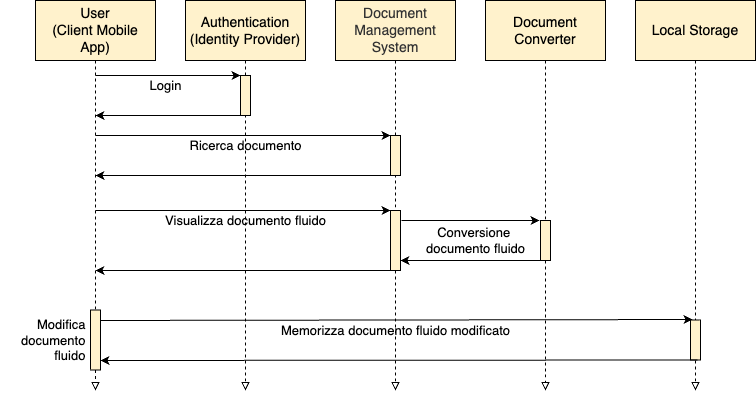
\includegraphics[width=1\textwidth]{img/tesi-2-Use-case2.drawio.png}
                \end{figure}
            \end{column}
            \begin{column}{0.4\textwidth}
                \begin{figure}[H]
                \centering
                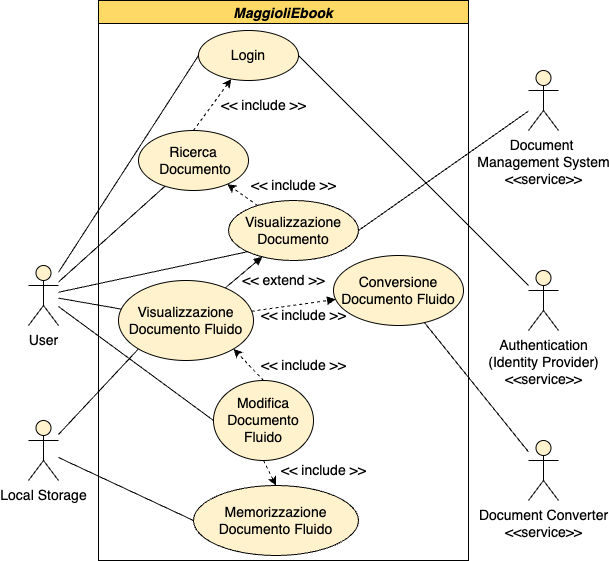
\includegraphics[width=1\textwidth]{img/tesi-1-Use-case.drawio.png}
                \end{figure}
            \end{column}
        \end{columns}
    \end{frame}

    \begin{frame}{Modellazione del dominio}
        \begin{columns}[onlytextwidth]
            \begin{column}{0.45\textwidth}
            \begin{itemize}
                \item Bounded Context:
                    \begin{itemize}
                        \item \textit{Reader} (Core) - Aspetti di maggiore valore per l'utente.
                        \item \textit{Sisred} - Sorgente delle pubblicazioni digitali Maggioli.
                        \item \textit{User} - Gestione delle identità e autenticazione.
                    \end{itemize}
                \item Relazioni Shared Kernel (SK) tra i contesti.
                \end{itemize}
            \end{column}
            \begin{column}{0.55\textwidth}
                \begin{figure}[H]
                \centering
                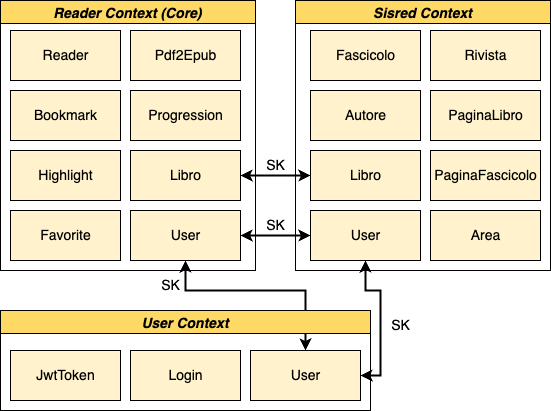
\includegraphics[width=0.9\textwidth]{img/tesi-20-app-domain.drawio.png}
                \end{figure}
            \end{column}
        \end{columns}
    \end{frame}

    \begin{frame}{Clean Architecture}
        \begin{columns}[onlytextwidth]
            \begin{column}{0.45\textwidth}
            \begin{itemize}
                \item Layers:
                    \begin{itemize}
                        \item \textit{Data} - Aggregati di dominio e gestione dati su differenti sorgenti.
                        \item \textit{Domain} - Casi d’uso del sistema che gestiscono il flusso dei dati da o verso il \textit{Data Layer}.
                        \item \textit{View} - UI e gestione eventi provenienti dall’utente o dal sistema.
                    \end{itemize}
                \end{itemize}
            \end{column}
            \begin{column}{0.55\textwidth}
                \begin{figure}[H]
                \centering
                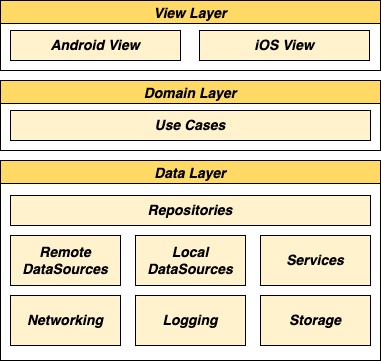
\includegraphics[width=0.8\textwidth]{img/tesi-2-Page-18.drawio.png}
                \end{figure}
            \end{column}
        \end{columns}
    \end{frame}
\end{document}
